% ----------------------------------------------------------
% DEFINITION
% ----------------------------------------------------------
\section{Definition}

The Readiness Adjustment Layer (RAL) is defined as a deterministic operator that
maps a baseline forecast to an adjusted forecast in order to reduce
decision-relevant loss under asymmetric cost and readiness constraints. Let
\(\yhat\) denote a baseline forecast generated by an arbitrary forecasting model,
and let \(\yhatadj\) denote the adjusted forecast produced by RAL. The adjustment
process is expressed as an operator
\[
\yhatadj = \RALop(\yhat),
\]
where \(\RALop\) applies a bounded transformation to \(\yhat\) without modifying
the underlying forecasting model or its parameters.

\subsection{Inputs}

RAL operates on the following inputs:
\begin{itemize}[leftmargin=*]
    \item \textbf{Baseline forecast} \(\yhat\), representing the original
    predictive estimate prior to any readiness-based adjustment.
    \item \textbf{Adjustment bounds} \(\deltaset = [\deltamin, \deltamax]\),
    defining the feasible range of forecast adjustments permitted by operational
    constraints.
    \item \textbf{Decision-oriented loss function} \(\CWSL(\cdot)\), which encodes
    asymmetric cost associated with over- and under-forecasting.
\end{itemize}

The feasible adjustment set \(\deltaset\) is externally specified and reflects
context-dependent limits such as capacity flexibility, buffer availability, or
policy-imposed guardrails. RAL does not infer or learn these bounds; it treats them
as fixed constraints.

\subsection{Adjustment Rule}

Conceptually, RAL evaluates adjusted forecasts of the form
\[
\yhatadj = \yhat + \delta, \quad \delta \in \deltaset,
\]
and selects an adjustment that minimizes decision-relevant loss. Formally,
\[
\yhatadj
=
\yhat + \argmin_{\delta \in \deltaset}
\CWSL(\yhat + \delta).
\]

In practice, forecast adjustments may be expressed either additively or
multiplicatively. The implementation described in this note uses bounded
\emph{multiplicative uplift factors}, which preserve non-negativity and relative
ordering of forecasts while operating within a predefined feasibility envelope.
The additive formulation above should therefore be interpreted as a conceptual
abstraction rather than a restriction on implementation.

When evaluated over a collection of forecast intervals \(t \in \Tset\), the
objective may be applied elementwise or in aggregate, depending on the operational
context, but the adjustment remains bounded within the feasible set for all
intervals.

% ----------------------------------------------------------
% FIGURE: RAL UPLIFT TRADEOFF CURVES
% ----------------------------------------------------------
\begin{figure}[htbp]
\centering
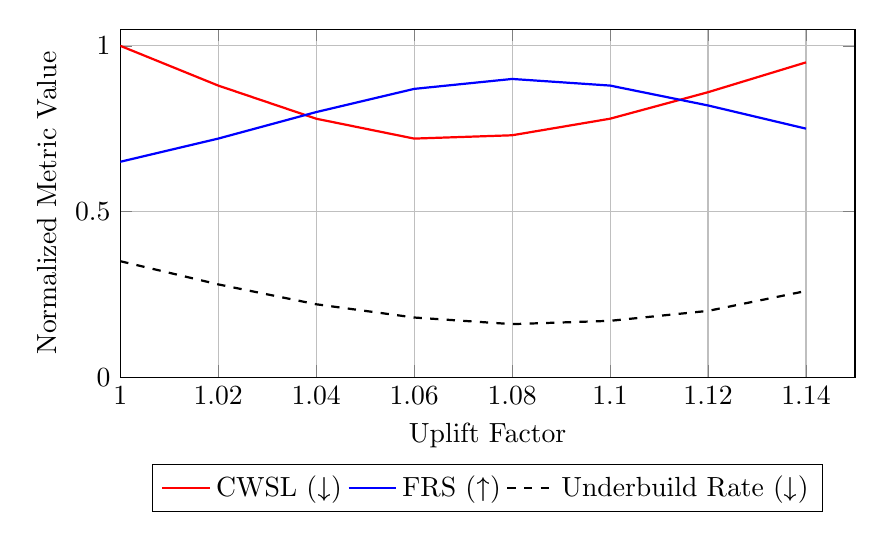
\begin{tikzpicture}
\begin{axis}[
    width=0.9\textwidth,
    height=6cm,
    xlabel={Uplift Factor},
    ylabel={Normalized Metric Value},
    xmin=1.0, xmax=1.15,
    ymin=0, ymax=1.05,
    legend style={at={(0.5,-0.25)}, anchor=north, legend columns=3},
    grid=major,
]

% CWSL (lower is better)
\addplot[thick, red]
coordinates {
    (1.00, 1.00)
    (1.02, 0.88)
    (1.04, 0.78)
    (1.06, 0.72)
    (1.08, 0.73)
    (1.10, 0.78)
    (1.12, 0.86)
    (1.14, 0.95)
};
\addlegendentry{CWSL (↓)}

% FRS (higher is better)
\addplot[thick, blue]
coordinates {
    (1.00, 0.65)
    (1.02, 0.72)
    (1.04, 0.80)
    (1.06, 0.87)
    (1.08, 0.90)
    (1.10, 0.88)
    (1.12, 0.82)
    (1.14, 0.75)
};
\addlegendentry{FRS (↑)}

% Underbuild Rate (lower is better)
\addplot[thick, dashed, black]
coordinates {
    (1.00, 0.35)
    (1.02, 0.28)
    (1.04, 0.22)
    (1.06, 0.18)
    (1.08, 0.16)
    (1.10, 0.17)
    (1.12, 0.20)
    (1.14, 0.26)
};
\addlegendentry{Underbuild Rate (↓)}

\end{axis}
\end{tikzpicture}
\caption{
Illustrative tradeoffs between cost-weighted service loss (CWSL),
Forecast Readiness Score (FRS), and underbuild rate as a function of
the uplift factor within a bounded feasibility envelope.
}
\label{fig:ral_uplift_tradeoff}
\end{figure}

The tradeoffs induced by the adjustment rule are illustrated in
Figure~\ref{fig:ral_uplift_tradeoff}. As the uplift factor varies within the
feasible envelope, cost-weighted service loss, forecast readiness, and
underbuild rate respond differently and exhibit opposing trends. Moderate
uplift reduces underbuild frequency and improves readiness, yielding a
corresponding reduction in decision-relevant loss. Beyond this region,
additional uplift increases overbuild cost and degrades overall performance.

RAL selects an operating point within this tradeoff surface that reduces
decision-relevant loss while preserving readiness and limiting adverse side
effects, rather than optimizing any single metric in isolation.

\subsection{Identity Condition}

If no adjustment within the feasible set produces a reduction in cost-weighted
service loss, RAL defaults to the identity transformation,
\[
\yhatadj = \yhat.
\]
This condition ensures that RAL cannot degrade performance relative to the
baseline forecast under the specified loss function and constraints.

\subsection{Outputs}

The primary output of RAL is the adjusted forecast \(\yhatadj\). In addition,
RAL produces diagnostic quantities used for evaluation and audit, including:
\begin{itemize}[leftmargin=*]
    \item Change in loss,
    \(\DeltaCWSL = \CWSL(\yhatadj) - \CWSL(\yhat)\).
    \item Change in Forecast Readiness Score (FRS), capturing improvements in
    readiness under asymmetric cost.
    \item Changes in under-readiness indicators, such as the underbuild rate
    \(\UBR\).
\end{itemize}

In addition to loss reduction, these diagnostics enable multi-metric audit of
readiness improvement and potential side effects, ensuring that RAL enhances
operational readiness rather than exploiting a single loss function. The
availability of parallel loss, readiness, and underbuild signals preserves
interpretability, supports governance review, and provides traceability for
downstream decision-making.